\documentclass{standalone}

\usepackage{tikz}

\begin{document}
	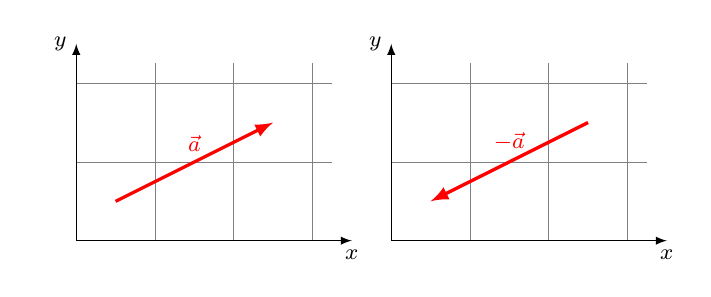
\begin{tikzpicture}
		[
		x=1cm, y=1cm, scale=1.0, font=\footnotesize, >=latex 
		%Voreinstellung für Pfeilspitzen
		]
		
		%Raster links im Hintergrund
		\draw[step=1, gray, very thin] (0,0) grid (3.25,2.25);
		
		%Länge x Achse
		\draw [-latex] (0,0) -- ++(3.5,0) node[below] {$x$};
		
		%Länge y Achse
		\draw [-latex] (0,0) -- ++(0,2.5) node[left] {$y$};	
		
		%Vektor a
		\draw[-latex, red, very thick] (0.5,0.5) -- ++(2,1) node [midway, above] {$\vec{a}$} node (a) {}; 
		
		\draw[dashed] (a.center) ++ (-3,0) node (c) {};
		
		%Raster links im Hintergrund
		\draw[step=1, gray, very thin] (4,0) grid (7.25,2.25);
		
		%Länge x Achse
		\draw [-latex] (4,0) -- ++(3.5,0) node[below] {$x$};
		
		%Länge y Achse
		\draw [-latex] (4,0) -- ++(0,2.5) node[left] {$y$};	
		
		%Vektor a
		\draw[-latex, red, very thick] (6.5,1.5) -- ++(-2,-1) node [midway, above] {$-\vec{a}$} node (a) {}; 
		
	\end{tikzpicture}
\end{document}